\section{Algorytm Gaussa-Legendre'a}

Algorytm Gaussa-Legendre'a jest aktualnie jednym z najszybciej zbiegających algorytmów używanych do wyliczania liczb $\pi$. Został wyprowadzony na podstawie prac Carla Friedricha Gaussa oraz Adrien-Marie Legendre na podstawie współczesnych algorytmów do mnożenia i pierwiastkowania.Jest on, niestety, bardzo wymagający pamięciowo. Poniżej prezentujemy implementację tego algorytmu\cite{gausse2}:

\newpage

\begin{lstlisting}[language=ps]
function gauss_legrendre (max):
    a = 1
    b = 1 / sqrt(2)
    t = 1 / 4
    p = 1
    i = 0
    while i <= max:
        an = (a + b) / 2
        b = sqrt(a * b)
        t = t - p * (a - an) * (a - an)
        p = 2 * p
        a = an
    
    return (a + b) * (a + b) / (4 * t)
\end{lstlisting}

\subsection{Wyniki}

Metoda Gaussa-Legrendre'a okazała się zbiegać do implementacji bibliotecznej funkcji \verb+pi()+ z języka \verb+Julia+ wyjątkowo szybko, bo już w 11 iteracji kwadrat błędu maszynowo był równy zeru, co widać na Wykresie~\ref{gauss-error}.

\begin{figure}[!h]
    \centering
    \renewcommand{\figurename}{Wykres}
    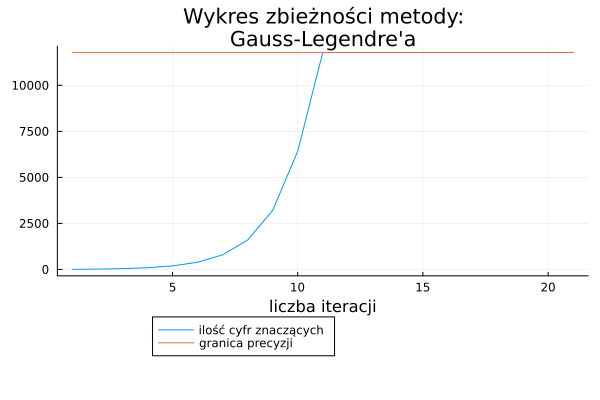
\includegraphics[width=0.7\textwidth]{../prog/gauss_legendre_log_error.png}
    \caption{Wykres ilości cyfr znaczących uzyskanych dla przybliżenia  $\pi$ za pomocą algorytmu Gaussa-Legendre'a.}
    \label{gauss-error}
\end{figure}

\begin{figure}[!h]
    \centering
    \renewcommand{\figurename}{Wykres}
    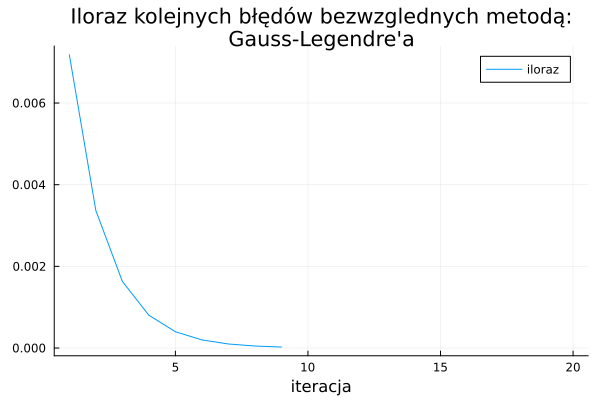
\includegraphics[width=0.7\textwidth]{../prog/gauss_legendre_error_ratio.png}
    \caption{Wykres ilorazu błędów względnych wyrazu $n+1$ i $n$ dla algorytmu Gaussa-Legrendre'a.}
    \label{gauss-convergence}
\end{figure}

Eksperymentalne obliczenia rzędu zbieżności tej metody jedynie potwierdzają wyższą zbieżność tego algorytmu niż w przypadku innych opisanych metod (Wykres~\ref{gauss-convergence}). Dla precyzji wynoszącej 16 069 bitów obliczenia na podstawie dzielenia błędu $(n+1)$-ego wyrazu przez kwadrat błędu $n$-tego wyrazu nie dają konkretnych wyników przez zbyt szybkie dążenie tej metody do $\pi$. W literaturze metoda ta jest określana jako zbieżna kwadratowo \cite{gausse-smth}.

Pomimo tak dobrej zbieżności, metoda ta nie jest powszechnie wykorzystywana, gdyż zużywa więcej pamięci niż metoda Chudnowskych.

\newpage

Wartość $\pi$ obliczona dla 10 iteracji naszego programu daje:

{\scriptsize
3.14159265358979323846264338327950288419716939937510582097494459230781640628620899862803482534211706798214808651\\
32823066470938446095505822317253594081284811174502841027019385211055596446229489549303819644288109756659334461284756\\
4823378678316527120190914564856692346034861045432664821339360726024914127372458700660631558817488152092096282925409\\
171536436789259036001133053054882046652138414695194151160943305727036575959195309218611738193261179310511854807446\\
2379962749567351885752724891227938183011949129833673362440656643086021394946395224737190702179860943702770539217176\\
2931767523846748184676694051320005681271452635608277857713427577896091736371787214684409012249534301465495853710507\\
9227968925892354201995611212902196086403441815981362977477130996051870721134999999837297804995105973173281609631859\\
50244594553469083026425223082533446850352619311881710100031378387528865875332083814206171776691473035982534904287554\\
68731159562863882353787593751957781857780532171226806613001927876611195909216420198938095257201065485863278865936153\\
38182796823030195203530185296899577362259941389124972177528347913151557485724245415069595082953311686172785588907509\\
83817546374649393192550604009277016711390098488240128583616035637076601047101819429555961989467678374494482553797747\\
26847104047534646208046684259069491293313677028989152104752162056966024058038150193511253382430035587640247496473263\\
91419927260426992279678235478163600934172164121992458631503028618297455570674983850549458858692699569092721079750930\\
29553211653449872027559602364806654991198818347977535663698074265425278625518184175746728909777727938000816470600161\\
45249192173217214772350141441973568548161361157352552133475741849468438523323907394143334547762416862518983569485562\\
09921922218427255025425688767179049460165346680498862723279178608578438382796797668145410095388378636095068006422512\\
52051173929848960841284886269456042419652850222106611863067442786220391949450471237137869609563643719172874677646575\\
73962413890865832645995813390478027590099465764078951269468398352595709825822620522489407726719478268482601476990902\\
64013639443745530506820349625245174939965143142980919065925093722169646151570985838741059788595977297549893016175392\\
84681382686838689427741559918559252459539594310499725246808459872736446958486538367362226260991246080512438843904512\\
44136549762780797715691435997700129616089441694868555848406353422072225828488648158456028506016842739452267467678895\\
25213852254995466672782398645659611635488623057745649803559363456817432411251507606947945109659609402522887971089314\\
566913686722874894056010150330861792868092087476091782493858900971490967598526136554978189312978482168299894872...
}